\documentclass[10pt,a4paper]{article}
%\usepackage[utf8]{inputenc}
\usepackage{fontspec}
\usepackage[polish]{babel}
\usepackage{amsmath}
%\usepackage{amsfonts}
%\usepackage{amssymb}
%\usepackage{makeidx}
%\usepackage{graphicx}
%\usepackage{mathtools}
\usepackage[left=2cm,right=2cm,top=2cm,bottom=2cm]{geometry}
\usepackage[colorlinks]{hyperref}
\usepackage{todonotes}
\usepackage{listings}
\usepackage{graphicx}
\usepackage{float}
\floatstyle{boxed}
\restylefloat{figure}
\usepackage{tikz}
\usepackage[europeanresistors,americaninductors]{circuitikz}



\author{Piotr Miedzik}
\title{MOZA - Projekt 1F07}
\makeindex
\begin{document}
\maketitle

\listoftodos
\section{Projekt}


Dla wzmacniacza szerokopasmowego jak na rysunku dobierz optymalizacyjne wartości Vdc, RF i CF tak by uzyskać maksymalną wartość GBW,
t.j. iloczynu wzmocnienia dla małych częstotliwości oraz 3dB górnej częstotliwości granicznej.
Określ wrażliwość funkcji celu na zmiany wartości rezystorów (w optimum).
Na tej podstawie oszacuj wariancję GBW spowodowaną przez losowe rozrzuty rezystorów o tolerancji 5\%.
Porównaj uzyskany wyniki ze statystykami obliczonymi przez symulację Monte Carlo.
Rozważ dwa przypadki rozrzutów rezystorów:
\begin{itemize}
\item rozrzuty nieskorelowane
\item rozrzuty skorelowane (współczynnik korelacji każdej pary rezystorów = 0.7)
\end{itemize}

\begin{figure}[H]
  \caption{Schemat układu}
  \centering
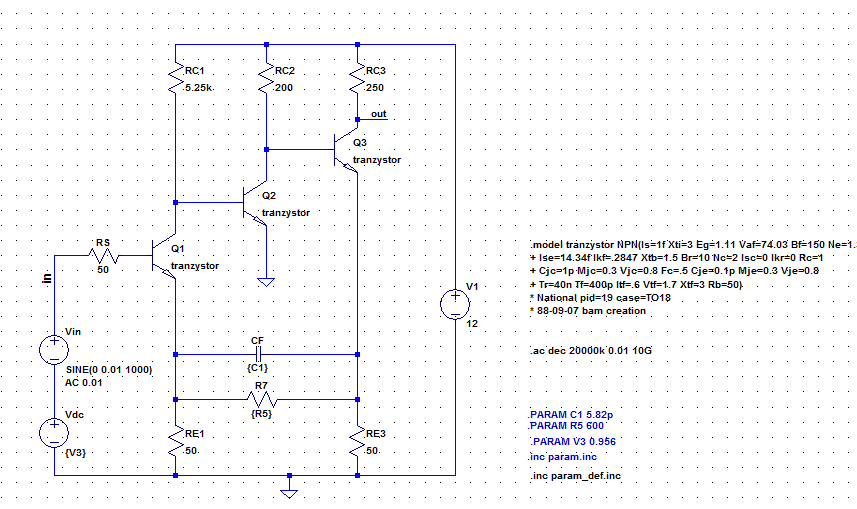
\includegraphics[scale=0.5]{obrazki/schemat2.png}
  \label{fig:schemat_ukladu}
\end{figure}


\section{Zadanie optymalizacji}
Zadanie polega na uzyskaniu możliwie najlepszej wartości GBW, poprzez optymalny dobór wartości RF, CF oraz napięcia Vdc.

\section{Wykonanie zadania}

W zadaniu nie określono wartości rezystora RC2 oraz maksymalnej amplitudy sygnału AC.
Wybrano przykładową wartość RC2 o wartości 200 Ohm oraz amplitudę 10mV (20mVpp).
Poprawność dobranych elementów sprawdzono za pomocą symulacji TRAN.
Kształt sygnału wyjściowego nie był zniekształcony.

\begin{figure}[H]
  \caption{Schemat układu}
  \centering
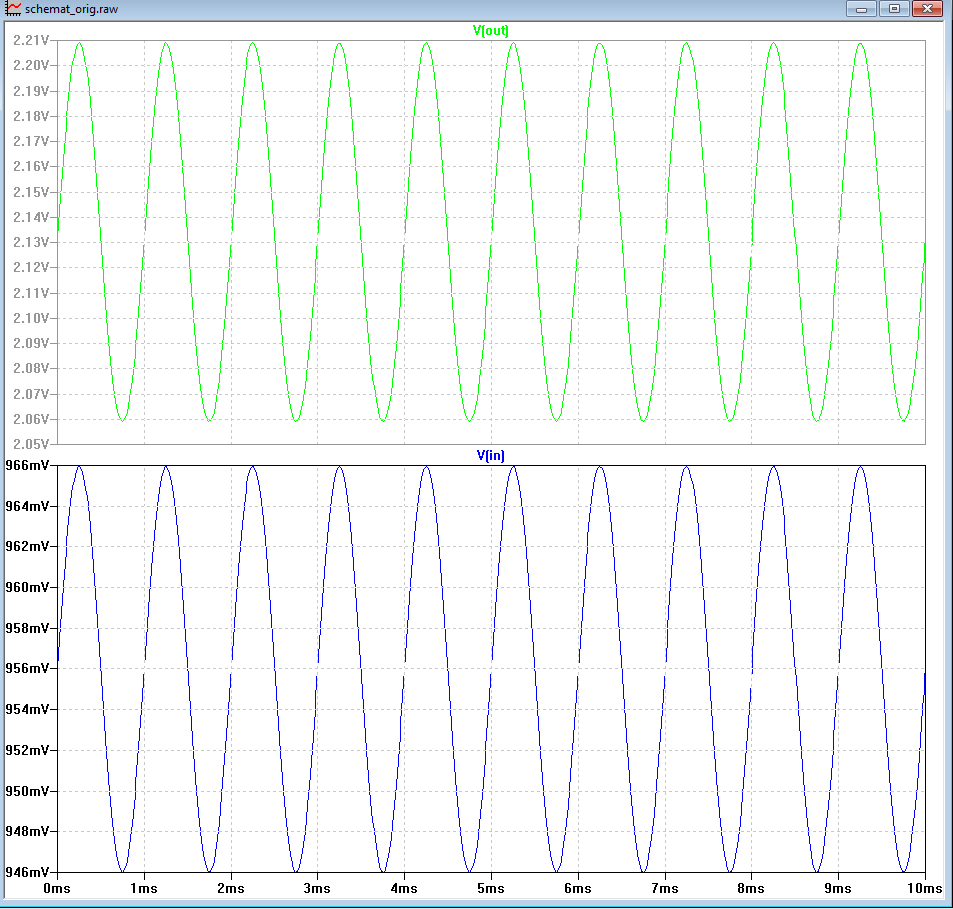
\includegraphics[scale=0.5]{obrazki/tran.png}
  \label{fig:schemat_tran}
\end{figure}

Za pomocą środowiska LTSpice, przeprowadzone zostały wstępne symulacje działania układu.
Określono wzmocnienie na poziomie 18.3dB (9.35586) oraz górną częstotliwość graniczną ok. 14.7Mhz.

$ GBW = 8.22992 * 14.7Mhz = 120,54M $

\todo[inline]{Wkleić charakterystykę AC}
\todo[inline]{Wkleić OP}

Określono również punkt pracy układu z wartościami początkowymi elementów.

\section{Funkcja celu}
Zadanie polega na uzyskaniu możliwie dużego iloczynu wzmocnienia dla małych częstotliwości oraz górnej częstotliwości granicznej.
Ponieważ metody wykorzystujące zadane algorytmy optymalizacji poszukują minimum funkcji dlatego też funkcja celu wygląda następująco:

$ f_c = -k_u * f_{g3dB} $

\section{Wykonanie zadania}

Zadanie wykonano przy użyciu środowiska Matlab oraz LTSpice. W środowisku Matlab zaimplementowano funkcję celu. Przy użyciu LTSpice natomiast symulowano kolejne parametry zaproponowane przez optymalizator. W każdym kolejnym wywołaniu funkcji celu obliczane były nowe wartości wzmocnienia dla małych częstotliwości i górnej częstotliwości granicznej, na podstawie współrzędnych charakterystyki częstotliwościowej przekazywanych do środowiska Matlab w postaci wyników symulacji LTSpice.

\section{Optymalizacja algorytmem Nelder - Mead}

Algorytm znalazł minimum funkcji celu po 100 iteracjach w których łącznie wywołał 201 razy funkcję celu.
Poniżej zamieszczono wykres przedstawiający wartość funkcji celu w zależności od iteracji.

\begin{figure}[H]
  \caption{Wykres wartości funkcji celu w funkcji iteracji}
  \centering
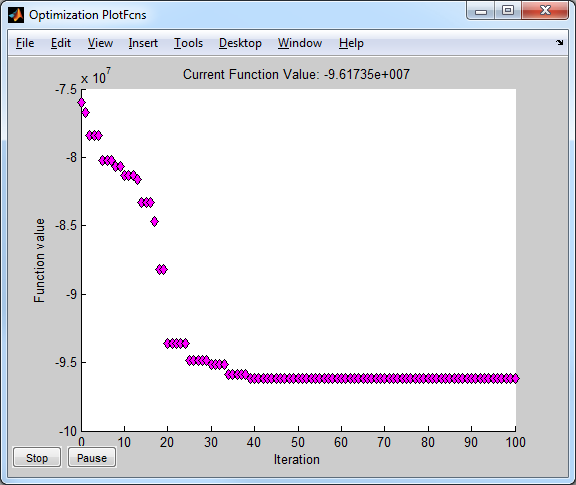
\includegraphics[scale=0.7]{obrazki/NF.png}
  \label{fig:schemat_tran}
\end{figure}

Można zauważyć, że od około 40 iteracji wartość funkcji celu zmieniała się już nieznacznie.
Istnieje więc możliwość skrócenia czasu pracy algorytmu, zgadzając się jednoczenie na nieco gorsze parametry.
Wartość minimalna funkcji celu jaką otrzymał optymalizator to -9.61735e+007.
Wartości elementów zamieszczono w tabeli poniżej.

\begin{tabular}{|c|c|}
\hline 
R5 & 703.486 \\ 
\hline 
C1 & 6.57504e-018 \\ 
\hline 
V3 & 1.01969 \\ 
\hline 
\end{tabular} 

Dla przedstawionych wartości przeprowadzono symulację w środowisku LTSpice, w celu porównania wyników z wartościami początkowymi.

$ k_u = 25dB = 9.3222 V/V  $

$ f_{3gdB} = 17.6Mhz  $

$ GBW = k_u * f_{3gdB} = 164M  $


\begin{tabular}{|c|c|c|}
\hline 
• & Przed optymalizacją & Po optymalizacji \\ 
\hline 
$ k_u $ & 8.2V/V & 9.3V/V \\ 
\hline 
$ f_{3gdB} $ & 14.7Mhz & 17.6Mhz \\ 
\hline 
$ GBW $ & 120,24M & 164M \\ 
\hline 
\end{tabular} 

\todo[inline]{Wkleić charakterystykę AC}
\todo[inline]{Wkleić wartości}

Podsumowując wyniki dla po przeprowadzeniu optymalizacji algorytmem NM udało się zwiększyć oczekiwaną wartość.
Dla nowych parametrów wzmacniacz ma lepsze wzmocnienie, oraz wzrosła wartość górnej częstotliwości granicznej.
%Nieznacznie również oddalono się od nasycenia w przypadku tranzystora Q1 ale też zbliżono się dla tranzystora Q3.


\section{Określenie wrażliwości funkcji celu}

\section{Porównanie z metoda Monte-Carlo}

\begin{verbatim}
mu = 50
sigma = 5
M = mu + sigma*randn(1000,2);
R = [1 0.75; 0.75 1];
L = chol(R)
M = M*L;
x = M(:,1);
y = M(:,2);
corr(x,y)
\end{verbatim}


\end{document}

Zadanie polegało na przeprowadzeniu analizy OP oraz AC przedstawionego poniżej układu wtórnika zbudowanego w oparciu o tranzystory NPN.
Analiza została wykonana w matlab’ie oraz dla sprawdzenia poprawności powtórzona Ltspice.

\begin{figure}[H]
  \caption{Schemat układu}
  \centering
    \includegraphics[scale=0.2]{images/schemat}
  \label{fig:schemat_ukladu}
\end{figure}

\begin{align}
V_{in} &= 
\begin{cases} 
1.5V, & \mbox{OP}\\
1, & \mbox{AC}
\end{cases}\\
Vee &= 12V\\
RB &= 1kOhm \\
RE &= 100kOhm
\end{align}


\subsection{Parametry tranzystora}

Na rysunku \ref{fig:tranzystor_ebers} został przedstawiony model tranzystora Ebersa Molla.
Następnie wstawiono równania opisujące poszczególne gałęzie oraz podano wartości parametrów.
\begin{figure}[H]
  \caption{Tranzystor wg modelu Ebersa Molla}
  \centering
    \includegraphics[scale=0.2]{images/ebers}
  \label{fig:tranzystor_ebers}
\end{figure}

\[
i_B = \frac{I_S}{BF} \left( exp \left(\frac{u_{BE}}{NFU_T} \right) - 1 \right) +
\frac{I_S}{BR} \left( exp \left(\frac{u_{BC}}{NRU_T} \right) - 1 \right)
\]
\[
i_C = I_S \left( exp \left(\frac{u_{BE}}{NFU_T} \right) - exp \left(\frac{u_{BC}}{NRU_T} \right) \right) -
\frac{I_S}{BR} \left( exp \left(\frac{u_{BC}}{NRU_T} \right) - 1 \right)
\]
\[
C_{BE} = \frac{TF\left( 1 + \frac{1}{BF} \right)I_S}{NFU_T} exp \left(\frac{u_{BE}}{NFU_T} \right) +
\frac{C_{jE0}}{{\left( 1 - \frac{\u_{BE}}{VJE} \right)}^{MJE}}
\]
\[
C_{BC} = TR \frac{I_S}{NRU_T} exp \left(\frac{u_{BC}}{NRU_T} \right) +
\frac{C_{jC0}}{{\left( 1 - \frac{\u_{BC}}{VJC} \right)}^{MJC}}
\]

Parametry modeli tranzystorów zostały dobrane zgodnie z poniższą tabelą.

\begin{tabular}{|c|c|}
\hline 
Symbol & Wartość \\ 
\hline 
IS & 1e-15[A] \\ 
\hline 
BF & 150 \\ 
\hline 
BR & 10 \\ 
\hline 
NF & 1 \\ 
\hline 
NR & 1 \\
\hline 
RB & 50Ohm \\ 
\hline 
TF & 400ps \\ 
\hline 
TR & 40ns \\ 
\hline 
CJC & 1pF \\ 
\hline 
CJE & 0.1pF \\ 
\hline 
VJC & 0.8 \\ 
\hline 
VJE & 0.8 \\ 
\hline 
MJC & 0.3 \\ 
\hline 
MJE & 0.3 \\ 
\hline 
UT & 25mV \\ 
\hline 
\end{tabular} 
\begin{figure}[H]
  \caption{Schemat zastępczy}
  \centering
    \includegraphics[scale=0.2]{images/schemat_zastepczy}
  \label{fig:schemat_zastepczy}
\end{figure}

Na schemacie zastępczym (Rysunek \ref{fig:schemat_zastepczy}) uwzględniono model tranzystora Ebersa Molla,
Ponumerowano węzły, zaznaczono napięcia.  


\section{Analiza OP}
\subsection{Schemat zastępczy dla analizy OP}

W analizie OP wszystkie pojemności zastępujemy rozwarciem, wszystkie źródła napięcia zmiennego i indukcyjności zwieramy.
Rezystancje warto zamienić na przewodności.

\[
E_{1} = 1.5V
\]
\[
E_{10} = 12V
\]
\[
G_{2} = \frac{1}{RB}
\]
\[
G_{3} = \frac{1}{R_{B3}}
\]
\[
G_{11} = \frac{1}{R_{B11}}
\]
\[
G_{18} = \frac{1}{R_{e}}
\]


\begin{figure}[H]
  \caption{tranzystor zlinearyzowany na na potrzeby analizy OP}
  \centering
\includegraphics{schemat.png}
    \includegraphics[scale=0.2]{images/linearyzacja_op}
  \label{fig:linearyzacja OP}
\end{figure}

Kolejnym krokiem jest linearyzacja elementów nieliniowych:

Dla gałęzi ic:
\[
i_{c}^{(p+1)}= g_{be}^{(p)} \left( v_{B'}^{(p+1)} - v_E^{(p+1)} \right) +
 g_{bc}^{(p)} \left( v_{B'}^{(p+1)} - v_C^{(p+1)} \right) + j_{c}^{(p)}
\]
\[
g_{be}^{(p)} = \frac{I_S}{NF \cdot U_T} \cdot exp \left( \frac{v_{B'}^{(p)} - v_E^{(p)}}{NF \cdot U_T} \right)
\]
\[
g_{bc}^{(p)} = 
- \frac{I_S}{NR \cdot U_T} \cdot exp \left( \frac{v_{B'}^{(p)} - v_C^{(p)}}{NR \cdot U_T} \right)
- \frac{I_S}{BR \cdot NR \cdot U_T} \cdot exp \left( \frac{v_{B'}^{(p)} - v_C^{(p)}}{NR \cdot U_T} \right)
\]

\[
j_{c}^{(p)} = I_S \left( exp \left(  \frac{v_{B'}^{(p)} - v_E^{(p)}}{NF \cdot U_T} \right) 
-exp \left( \frac{v_{B'}^{(p)} - v_C^{(p)}}{NR \cdot U_T} \right)
\right) -
\frac{I_S}{BR} \left( exp \left( \frac{v_{B'}^{(p)} - v_C^{(p)}}{NR \cdot U_T} \right) - 1 \right) - g_{be}^{(p)} \left( v_{B'}^{(p)} - v_E^{(p)} \right) -
g_{bc}^{(p)} \left(v_{B'}^{(p)} -v_C^{(p)} \right)
\]
Dla gałęzi ib
\[
i_{b}^{(p+1)}= g_{be}^{(p)} \left( v_{B'}^{(p+1)} - v_E^{(p+1)} \right) +
 g_{bc}^{(p)} \left( v_{B'}^{(p+1)} - v_C^{(p+1)} \right) + j_{b}^{(p)}
\]
\[
g_{be}^{(p)} = \frac{I_S}{BF \cdot NF \cdot U_T} \cdot exp \left( \frac{v_{B'}^{(p)} - v_E^{(p)}}{NF \cdot U_T} \right)
\]
\[
G_{bc}^{(p)} = 
- \frac{I_S}{BR \cdot NR \cdot U_T} \cdot exp \left( \frac{v_{B'}^{(p)} - v_C^{(p)}}{NR \cdot U_T} \right)
\]

\[
j_{b}^{(p)} = \frac{I_S}{BF} \left( exp \left(  \frac{v_{B'}^{(p)} - v_E^{(p)}}{NF \cdot U_T} \right) 
- 1 \right) +
\frac{I_S}{BR} \left( exp \left( \frac{v_{B'}^{(p)} - v_C^{(p)}}{NR \cdot U_T} \right) - 1 \right) -
g_{be}^{(p)} \left( v_{B'}^{(p)} - v_E^{(p)} \right) -
G_{bc}^{(p)} \left(v_{B'}^{(p)} -v_C^{(p)} \right)
\]

\subsection{Rownania sieci OP}
\begin{align*}
 i_1 &= i_1 \\
 i_2 &= G_2 (V_1 - V_5) \\
 i_3 &= G_3 (V_5 - V_7) \\
 i_4 &= g_4 (V_7 - V_3) // g_{be}\\
 i_5 &= G_5 (V_7 - V_2) // G_{bc}\\
 i_6 &= j_6 \\
 i_7 &= g_7 (V_7 - V_3) // g_{be}\\
 i_8 &= g_8 (V_7 - V_2) // g_{bc} \\
 i_9 &= j_9 \\
i_{10} &= i_10 \\
i_{11} &= G_{11} (V_3 - V_6) \\
i_{12} &= g_{12} (V_6 - V_4) // g_{be}\\
i_{13} &= G_{13} (V_6 - V_2) // G_{bc}\\
i_{14} &= j_{14} \\
i_{15} &= g_{15} (V_6 - V_4) // g_{be}\\
i_{16} &= g_{16} (V_6 - V_2) // g_{bc}\\
i_{17} &= j_{17} \\
i_{18} &= G_{18} (V_4 - V_0)
\end{align*}

\subsection{Równania kanoniczne sieci OP}
\begin{align*}
V_1 :& i_1 + i_2 = 0\\
V_2 :& i_7 + i_8 + i_9 + i_{10} + i_{15} + i_{16} + i_{17} = 0 \\
V_3 :& -i_4 - i_5 - i_6 -i_7 -i_8 - i_9 + i_{11} = 0\\
V_4 :& -i_{12} -i_{13} -i_{14} -i_{15} -i_{16} -i_{17} +  i_{18} = 0\\
V_5 :& -i_{2} + i_{13} = 0\\
V_6 :& -i_{11} + i_{12} + i_{13} + i_{14} = 0\\
V_7 :& -i_{3} + i_{4} + i_{5} + i_{6} = 0\\
i_1 :& u_1 = V_1 - V_0 = e_1 \\
i_{10} :& u_{10} = V_2 - V_0 = V_{ee}
\end{align*}

\subsection{Równania sieci iteracyjnej w postaci macierzy}
\footnotesize
\begin{align*}
Y = 
\begin{bmatrix}
G_2 & 0 & 0 & 0 & -G_2 & 0 & 0 & 1 & 0 \\
0 & -g_8 -g_{16} & -g_7 & -g_{15} & 0 & g_{15} + g_{16} & g_7 + g_8 & 0 & 1 \\
0 & G_5+g_8 & g_4 + g_7 + G_{11} & 0 & 0 & -G_{11} & -g_4-G_5-g_7-g_8 &0 & 0 \\
0 & g_{16} + G_{13} & 0 & g_{12} + g_{15} + G_{18} & 0 & -g_{12} - G_{13} -g_{15} - g_{16} &0 &0 & 0 \\
-G_2 & 0 & 0 & 0 &G_2 +G_3 & 0 & -G_3 & 0 & 0 \\
0 & -G_{13} & -G_{11} & -g_{12} & 0& G_{11} + g_{12} + G_{13} & 0 &0 &0  \\
0 & -G_5 & -g_4 & 0 & -G_3 & 0 &G_3 + g_4 + G_5 &0 & 0 \\
1 &0 &0 &0 &0 &0 &0 &0 & 0 \\
0 &1 &0 &0 &0 &0 &0 &0 &0
\end{bmatrix}
\end{align*}
\normalsize

\begin{align*}
X = 
\begin{bmatrix}
V_1 \\
V_2 \\
V_3 \\
V_4 \\
V_5 \\
V_6 \\
V_7 \\
i_1 \\
i_{10}
\end{bmatrix}
\end{align*}

\begin{align*}
b = 
\begin{bmatrix}
0 \\
-j_9 - j_{17} \\
j_6 + j_9 \\
j_{14} + j_{17} \\
0 \\
-j_{14} \\
-j_6 \\
e_1 \\
V_{ee}
\end{bmatrix}
\end{align*}


\subsection{Symulacja w programie LT Spice}

\includegraphics{schemat.png}


\subsection{Porównanie symulacji LTSpice i Matlab}
\begin{tabular}{|p{8.5cm}|p{4.5cm}|p{2cm}|}
\hline 
LTSpice & Matlab & Błąd \\
\hline 
\begin{lstlisting}
       --- Operating Point ---

V(2):	 12	 voltage
V(5):	 1.49996	 voltage
V(3):	 1.00103	 voltage
V(4):	 0.432637	 voltage
V(1):	 1.5	 voltage
Ic(Q1):	 4.01568e-006	 device_current
Ib(Q1):	 3.10684e-007	 device_current
Ie(Q1):	 -4.32637e-006	 device_current
Ic(Q2):	 2.72276e-007	 device_current
Ib(Q2):	 3.84079e-008	 device_current
Ie(Q2):	 -3.10686e-007	 device_current
I(R2):	 -3.84079e-008	 device_current
I(R1):	 4.32637e-006	 device_current
I(V2):	 -4.28796e-006	 device_current
I(V1):	 -3.84079e-008	 device_current
\end{lstlisting}
& \begin{lstlisting}


V(2):  12
V(5):  1.5
V(3):  1.0514
V(4):  0.47244
V(1):  1.5






I(RB): 2.072e-010
I(RE): 4.7244e-006
\end{lstlisting}
& - \\ 
\hline 
\end{tabular} 


Algorytm zakończył pracę po 23 iteracjach.
Otrzymane wyniki porównano z wynikami symulacji programem Ltspice.
Ponieważ otrzymane wartości nie są równe, istnieje prawdopodobieństwo tego,
że symulacja w matlabie została błędnie zaprojektowana. 
Mogła też nastąpić gdzieś pomyłka przy przepisywaniu danych.
Innym potencjalnym powodem dla którego wyniki analizy OP są rozbieżne to użycie funkcji dxpo oraz expo, w których zastosowano pewne przybliżenia.
Jednak w analizie OP nie powinno mieć to aż takiego znaczenia.


\section{Analiza AC}

\begin{figure}[H]
  \caption{tranzystor zlinearyzowany na na potrzeby analizy AC}
  \centering
	\includegraphics[scale=0.2]{images/ebers}
    \includegraphics[scale=0.2]{images/linearyzacja_ac}
  \label{fig:linearyzacja OP}
\end{figure}

Na powyższym schemacie zastępczym źródła prądowe niezależne zastąpiono rozwarciami, a źródła napięciowe niezależne zostały zastąpione zwarciami. 
Ponadto wprowadzone zostały admitancje zastępujące pojemności występujące w tranzystorach bipolarnych. W analizie wykorzystano również elementy wyznaczone podczas analizy OP.
Analizę przeprowadzono dla zakresu od 1Hz do 1GHz. 

Ponieważ nieliniowe pojemności tranzystora bipolarnego są zdefiniowane w funkcji $C(v)$, admitancje przyjmują następujące wzory:
\begin{align}
Y19 = j*\omega*C\left(v_7 - v_2 \right)\\
Y20 = j*\omega*C\left(v_7 - v_3 \right)\\
Y21 = j*\omega*C\left(v_6 - v_2 \right)\\
Y22 = j*\omega*C\left(v_6 - v_4 \right)\\
\end{align}

\subsubsection{Rownania sieci AC}
\begin{align*}
 i_1 &= i_1 \\
 i_2 &= G_2 (V_1 - V_5) \\
 i_3 &= G_3 (V_5 - V_7) \\
 i_4 &= g_4 (V_7 - V_3) // g_{be}\\
 i_5 &= G_5 (V_7 - V_2) // G_{bc}\\
 i_20 &= Y_{20} (V_7 - V_3)\\
 i_19 &= Y_{19} (V_7 - V_2)\\
 i_7 &= g_7 (V_7 - V_3) // g_{be}\\
 i_8 &= g_8 (V_7 - V_2) // g_{bc} \\
i_{10} &= i_10 \\
i_{11} &= G_{11} (V_3 - V_6) \\
i_{12} &= g_{12} (V_6 - V_4) // g_{be}\\
i_{13} &= G_{13} (V_6 - V_2) // G_{bc}\\
i_22 &= Y_{20} (V_6 - V_4)\\
i_21 &= Y_{19} (V_6 - V_2)\\
i_{15} &= g_{15} (V_6 - V_4) // g_{be}\\
i_{16} &= g_{16} (V_6 - V_2) // g_{bc}\\
i_{18} &= G_{18} (V_4 - V_0)
\end{align*}

\subsubsection{Równania kanoniczne sieci AC}
\begin{align*}
V_1 :& i_1 + i_2 = 0\\
V_3 :& -i_4 - i_5 - i_20 -i_7 -i_8 + i_{11} = 0\\
V_4 :& -i_{12} -i_{13} -i_{22} -i_{15} -i_{16} +  i_{18} = 0\\
V_5 :& -i_{2} + i_{13} = 0\\
V_6 :& -i_{11} + i_{12} + i_{13} + i_{22} + i_{21} = 0\\
V_7 :& -i_{3} + i_{4} + i_{5} + i_{20} + i_{19}  = 0\\
i_1 :& u_1 = V_1 - V_0 = e_1 \\
\end{align*}

\subsection{Równania sieci AC w postaci macierzy}

\footnotesize
\begin{align*}
Y = 
\begin{bmatrix}
G2 & 0 & 0 & -G2 & 0 & 0 & 1 \\
0 & g4+Y20+g7+G11 & 0 & 0 & -G11 & -g4-G5-Y20-g7-g8 & 0\\
0 & 0 & g12+Y22+g15+G18 & 0 & -g12-Y22-G13-g15-g16 & 0 & 0\\
-G2 & 0 & 0 & G2+G3 & 0 & -G3 & 0\\
0 & -G11 & -g12-Y22 & 0 & G11+g12+G13+Y22+Y21 & 0 & 0\\
0 & -g4-Y20 & 0 & -G3 & 0 & G3+g4+G5+Y20+Y19 & 0\\
1 & 0 & 0 & 0 & 0 & 0 & 0
\end{bmatrix}
\end{align*}
\normalsize

\begin{align*}
X = 
\begin{bmatrix}
V_1 \\
V_3 \\
V_4 \\
V_5 \\
V_6 \\
V_7 \\
i_1
\end{bmatrix}
\end{align*}

\begin{align*}
b = 
\begin{bmatrix}
0 \\
0 \\
0 \\
0 \\
0 \\
0 \\
e_1
\end{bmatrix}
\end{align*}

\begin{figure}[H]
  \caption{schemat zlinearyzowany na na potrzeby analizy AC}
  \centering
    \includegraphics[scale=0.2]{images/zastepczy_ac}
  \label{fig:linearyzacja OP}
\end{figure}
\subsection{Porównanie wyników symulacji za pomocą Matlaba oraz LTspice}

\begin{figure}[H]
  \caption{LTSpice: charakterystyka amplitudowa i fazowa układu}
  \centering
    \includegraphics[scale=0.8]{../ltspice/ac}
  \label{fig:matlab_wzm_faza}
\end{figure}

\begin{figure}[H]
  \caption{Matlab: charakterystyka amplitudowa układu}
  \centering
    \includegraphics[scale=0.8,page=1,clip=true,trim=2cm 9.5cm 2cm 10cm]{../projekt1/wzmocnienie}
  \label{fig:matlab_wzm}
\end{figure}
\begin{figure}[H]
  \caption{Matlab: charakterystyka fazowa układu}
  \centering
    \includegraphics[scale=0.8,page=1,clip=true,trim=2cm 9.5cm 2cm 10cm]{../projekt1/fazowy}
  \label{fig:matlab_faza}
\end{figure}

Poniżej przedstawiono wartości odczytane z wykresów dla programu LTSpice oraz skryptu Matlabowego:

\begin{tabular}{|c|c|c|}
\hline 
Częstotliwość & LTSpice & Matlab \\ 
\hline 
10kHz & -0.9dB & -0.9dB \\ 
\hline 
100kHz & -0.9dB & -1.3dB \\ 
\hline 
1MHz & -1.3dB & -9.1dB \\ 
\hline 
10MHz & -9.2dB & -13.6dB \\ 
\hline 
100MHz & -13.5dB & -14.0dB \\ 
\hline 
\end{tabular} 

Na podstawie powyższych danych, widać że wartości wzmocnień są podobne dla obydwu przypadków.
Różnią się one zakresem częstotliwości. 
Częstotliwość graniczna zależy w głównej mierze od pojemności $C_be$, która tworzy filtr dolnoprzepustowy.

Charakterystyki fazowe również są podobne.

\section{Skrypt matlab}
\lstinputlisting[language=Matlab,frame=single,title=opac.m]{../projekt1/opac.m}
\lstinputlisting[language=Matlab,frame=single,title=expo.m]{../projekt1/expo.m}
\lstinputlisting[language=Matlab,frame=single,title=dxpo.m]{../projekt1/dxpo.m}
\lstinputlisting[language=Matlab,frame=single,title=cbc.m]{../projekt1/cbc.m}
\lstinputlisting[language=Matlab,frame=single,title=cbe.m]{../projekt1/cbe.m}
\lstinputlisting[language=Matlab,frame=single,title=gbebe.m]{../projekt1/gbebe.m}
\lstinputlisting[language=Matlab,frame=single,title=Gbebc.m]{../projekt1/Gbebc.m}
\lstinputlisting[language=Matlab,frame=single,title=gcebe.m]{../projekt1/gcebe.m} 
\lstinputlisting[language=Matlab,frame=single,title=gcebc.m]{../projekt1/gcebc.m}
\lstinputlisting[language=Matlab,frame=single,title=jbe.m]{../projekt1/jbe.m}
\lstinputlisting[language=Matlab,frame=single,title=jce.m]{../projekt1/jce.m}
\section{Symulacje za pomocą hAMSter}
W symulatorze hAMSter przeprowadzono symulacje czasowe dla sygnału:
\begin{equation*}
u_1(t)= 
\begin{cases} 1.5V & \text{gdy $t < 25ns$,}
\\
1.5V+sin(2\pi \cdot 1Gz\cdot t ) &\text{gdy $x\geq 25ns$.}
\end{cases}
\end{equation*}
Symulacje w symulatorze hamster początkowo próbowano przeprowadzić dla pełnego schematu zadanego wtórnika.
Jednak wyniki symulacji tego układu na różne sposoby należało odrzucić,
ponieważ uzyskiwane wartości napięć i prądów na poszczególnych elementach układu kłóciły się ze stanem wiedzy.
Zostały one przedstawione na rysunku \ref{fig:hamster_dwa_tranzystory}.
\begin{figure}[H]
  \caption{Napięcia na wybranych elementach przy pełnej konfiguracji}
  \centering
    \includegraphics[scale=0.4]{../hamster/dwa_tranzystory.png}
  \label{fig:hamster_dwa_tranzystory}
\end{figure}
Napięcie na rezystorze RE ($u_18$) wynosi 10,45V,a według przewidywań powinno ono wynosić około 0,4V.
Napięcie baza-emiter tranzystora dolnego ($u_be2$) wydaje się być prawidłowe,
ale napięcie baza-emiter tranzystora górnego ($u_be1$) wynosi -9,809V co jest oczywiście niemożliwe.

Postanowiono więc usunąć jeden z tranzystorów, tak aby przesymulować go w programie hAMSter i porównać wyniki z symulacjami w programie LTSpice.
Schemat przedstawiono na rysunku \ref{fig:ltspice_jeden_tranzystor}
\begin{figure}[H]
  \caption{Zmodyfikowany układ}
  \centering
    \includegraphics[scale=1]{../ltspice/ltspice_jeden_tranzystor.png}
  \label{fig:ltspice_jeden_tranzystor}
\end{figure}

\begin{figure}[h!]
  \caption{hAMSter: Napięcia na wybranych elementach przy pełnej konfiguracji}
  \centering
    \includegraphics[scale=0.4]{../hamster/jeden_tranzystor.png}
  \label{fig:hamster_jeden_tranzystor}
\end{figure}

\begin{figure}[h!]
  \caption{LTSpice: Wykres napięcia na rezystorze RE}
  \centering
    \includegraphics[scale=1]{../ltspice/wykres.png}
  \label{fig:ltspice_wykres}
\end{figure}

Na rysunkach \ref{fig:hamster_jeden_tranzystor} oraz \ref{fig:ltspice_wykres} przedstawiono wykresy napięć na wybranych elementach.
Z wykresów symulacji programem hAMSter wynika, że w punkcie pracy napięcie na rezystorze RE ($u_{18}$) wynosi 0,904V.
Maksymalne oraz minimalne napięcie na wykresie przebiegu czasowego wynosi odpowiednio: 1,219 oraz 0,589.

Z analizy OP programem LTSpice wnika natomiast, że w punkcie pracy na rezystorze RE napięcie wynosi 0,911V.
Maksymalne oraz minimalne napięcie na wykresie przebiegu czasowego wynosi natomiast: 1,227V oraz 0,595V.

\subsection{Uwagi do symulacji programem hAMSter}
Nie udało się zrealizować symulacji układu w konfiguracji zadanej w projekcie, 
pomimo tego że wszystkie elementy składowe (tranzystory, rezystory) osobno symulowane były prawidłowo.

Przed rozpoczęciem symulacji należy ustawić odpowiednio mały minimalny krok symulacji. W tym przypadku była to 1ps.

Wynikowe wartości napięcia i natężenia prądu na poszczególnych elementach zależą od długości kroku jaki będzie ustawiony w symulatorze (dotyczy to również programu LTSpice).

Analiza uproszczonego schematu przy częstotliwości 1GHz dały trochę inne rezultaty niż w programie LTspice.
Różnica w punkcie pracy może wynikać z tego, że w programie LTSpice nie znaleziono opcji temperatury symulacji, która wpływa na parametr Ut.
\section{Skrypt VHDL}
\lstinputlisting[language=vhdl,frame=single,title=dwa\_tranzystory.vhd]{../hamster/dwa_tranzystory.vhd}
\lstinputlisting[language=vhdl,frame=single,title=jeden\_tranzystor.vhd]{../hamster/jeden_tranzystor.vhd}

\end{document}